%% VISAP 2026 (Amplification) submission, Papers track.
%% Formatted with the IEEE VGTC conference class (vgtc.cls), the house style for
%% IEEE VIS-affiliated venues. Compile on Overleaf or any TeX Live install with:
%%   pdflatex -> bibtex -> pdflatex -> pdflatex
%% VISAP uses a SINGLE-BLIND review process, so author identities are retained.

\documentclass{vgtc}                          % final (conference) style

%% cross-references use cleveref (loaded automatically by the vgtc class).
\graphicspath{{figures/}{pictures/}{images/}{./}} % where to search for images

\usepackage{times}                     % Times as the main font
\renewcommand*\ttdefault{txtt}         % a nicer typewriter font
\usepackage{booktabs}                  % rules for the case-study table
\usepackage{amsmath}                   % the single (deliberately trivial) equation
\usepackage{mathptmx}                  % matching math font

%% single-blind review: no online id / anonymization needed
\onlineid{0}
\vgtccategory{Research}
\vgtcinsertpkg

%% Paper title.
\title{The Choreographic Genome:\\Amplifying the Silent Structure of Text into Dance}

%% Author and Affiliation (two authors, one affiliation).
\author{Michael Li\thanks{e-mail: ml7@andrew.cmu.edu}
\and Alison Ding\thanks{e-mail: alisondi@andrew.cmu.edu}}
\affiliation{\scriptsize Carnegie Mellon University}

%% Teaser figure across the top of the first page.
\teaser{
  \centering
  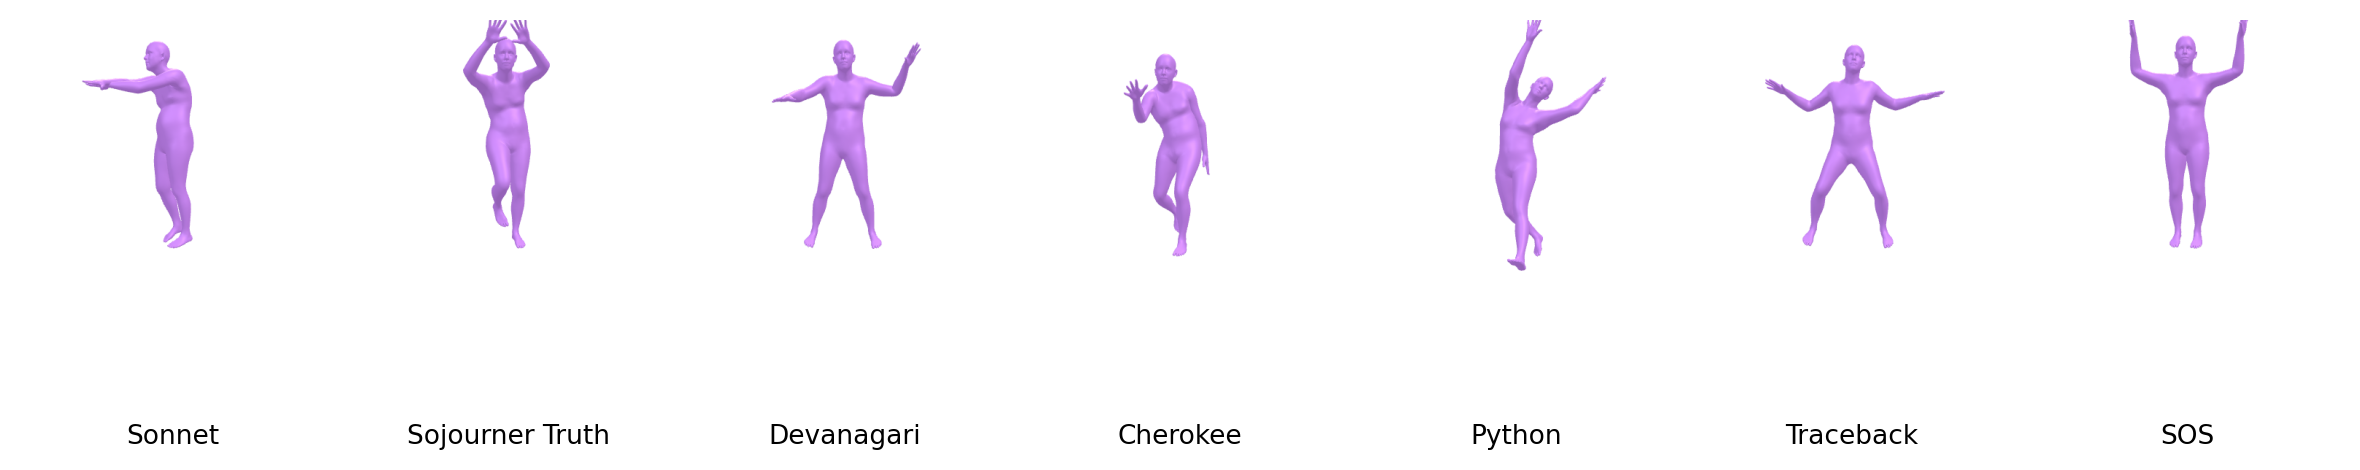
\includegraphics[width=\linewidth]{plot_8_teaser}
  \caption{Seven texts, seven bodies. A single expressive keyframe from the
  choreography our instrument generates for each case-study text, from a
  Shakespeare sonnet to an ``SOS'' in Morse. The mapping from text to movement
  never consults meaning, only structure, yet each text still produces a visibly
  distinct dance. Every body is rendered from the same underlying engine.}
  \label{fig:teaser}
}

%% Abstract.
\abstract{
Recent advances in generative artificial intelligence have enabled the synthesis
of complex human motion with unprecedented fidelity. However, current
text-to-motion systems rely strictly on linguistic semantics: if an input reads
``I put my hands up'', the model searches for a pose with raised hands, and every
non-semantic property of the text is discarded as noise. In this work, we treat
that discarded structure as the signal. We present an embodied visualization
instrument that amplifies not what a text means, but how it is built. Our method
first quantizes dance kinematics into a motion codebook of 256 stylistic
``regions'' using Principal Component Analysis and K-Means clustering. We then map
the raw byte representation of any input text directly onto this codebook,
producing a deterministic sequence of regions that we call the text's
``choreographic genome''. A precomputed plausibility graph and a set of physics
smoothing routines turn this genome into fluid, full-body movement, so that the
dancing body becomes a display surface for the byte-level structure that semantic
systems ignore. Through a series of artistic case studies, including a Shakespeare
sonnet, a machine error log, source code, an abolitionist's question, and
Indigenous and Devanagari scripts, we show that each text produces a visibly
distinct dance, and that scripts marginalized by ASCII-centric computing are
amplified into three to four times more movement per character. We frame this not
as a motion-synthesis benchmark, but as a critical and poetic visualization that
asks what we choose to count as signal, and what we allow to go unheard.
}

%% Keywords (optional for VISAP; included to aid reviewer matching).
\keywords{Amplification, embodied visualization, data physicalization, generative
art, motion synthesis, co-creation.}

%%%%%%%%%%%%%%%%%%%%%%%%%%%%%%%%%%%%%%%%%%%%%%%%%%%%%%%%%%%%%%%%
%%%%%%%%%%%%%%%%%%%%%% START OF THE PAPER %%%%%%%%%%%%%%%%%%%%%%
%%%%%%%%%%%%%%%%%%%%%%%%%%%%%%%%%%%%%%%%%%%%%%%%%%%%%%%%%%%%%%%%%

\begin{document}

\firstsection{Introduction}

\maketitle

While data permeates every aspect of our world, its representation is rarely equitable. Certain narratives are elevated to positions of influence, whereas others are left obscured, fractured, or intentionally suppressed~\cite{dignazio2020datafeminism,gitelman2013rawdata}. If visualization serves as a tool for amplification, bringing clarity to the quiet and presence to the ignored, we must critically examine how we wield it. In this paper, we explore this dynamic literally by interrogating our own creative systems: when we design a tool to magnify a specific signal, what exactly are we elevating, and what inadvertently gets muted?

Text is one of the most quietly structured data streams we produce. Every message
carries far more than its dictionary meaning; it carries an encoding, a
distribution of bytes, a choice of script, and a rhythm of repetition. However,
the dominant paradigm of generative artificial intelligence is built to hear only
one of these layers. Text-to-motion and text-to-image models treat the semantic
content of language as literal instruction, and they discard everything else as
noise~\cite{li2021aist,stanford2023edge}. For example, for typical choreography, if the lyrics say ``I put my hands up'', the model returns a figure with raised
hands. The structure of the language, which is the
actual material of it, is silenced in favor of its most sanctioned reading.

In this work, we present an embodied visualization instrument that inverts this
hierarchy. Rather than amplifying what a text means, we amplify how a text is
built. Our system reads the raw bytes of an input string and maps each byte
directly onto one of 256 quantized ``motion regions'', a learned vocabulary of
human movement. The resulting sequence is a deterministic structural fingerprint
that we call the text's ``choreographic genome'' (\cref{fig:genome}). A
precomputed plausibility graph then stitches the genome into biomechanically
continuous motion, and the dancing body becomes a display, a physical readout of
the byte-level structure that semantics-first systems throw away. Because the
mapping never consults meaning, every text, whether a sonnet, an error log, a
protest, a line of code, or a script that ASCII never planned for, is given a body
on equal terms (\cref{fig:teaser}).

We make three contributions. First, we reframe text-to-motion not as semantic
translation but as structural amplification, and we argue for the body as a
display surface for the otherwise invisible material of language
(\cref{sec:related,sec:system}). Second, we describe a fully functional and
interpretable pipeline, built on classical machine learning and graph search
rather than a black-box neural generator, that runs on a consumer CPU
(\cref{sec:system}). Third, through a set of artistic case studies over a
deliberately heterogeneous corpus, we show that the instrument gives each text a
visibly distinct dance, and that scripts marginalized by digital infrastructure
are amplified into three to four times more movement per character than ASCII
English (\cref{sec:cases}).

We do not position this work as a more accurate motion model; the merit of our engine should not be judged based on typical motion generation quality metrics such as foot-skating ratio or floor penetration rate. We instead position this work as a
critical and poetic visualization that uses generative technology to amplify the
quiet structure of our data streams, and that keeps an honest account of the
biases it introduces along the way.

\section{Related Work}
\label{sec:related}

\subsection{Dance generation and the semantic ceiling}
Current research in AI dance generation focuses primarily on the technical
challenge of synthesizing high-fidelity kinetic movement, often conditioned on
text or audio. Systems such as EDGE, Bailando, and DanceFormer have achieved
remarkable success in generating physically plausible motion that adheres to a
provided prompt~\cite{stanford2023edge,siyao2022bailando,li2023danceformer},
trained on datasets such as AIST++, GDANCE, and
FineDance~\cite{li2021aist,le2023gdance,li2023finedance}. However, these systems
inherently bind movement to the literal, semantic meaning of their inputs, and
they treat dance generation as a supervised translation of human intent into
physical space. This approach inherits the cultural and linguistic biases of the
training data~\cite{crawford2021atlas}, and it leaves a critical gap regarding how
a generative system might interpret text abstractly. Our instrument targets
exactly this gap: it treats text as a structural sequence of raw choreographic
tokens rather than as a set of instructions to be obeyed.

\subsection{Amplification and what counts as signal}
The premise that ``raw data'' is ever truly raw, rather than shaped by those who
collect and encode it, has been thoroughly
critiqued~\cite{gitelman2013rawdata,dignazio2020datafeminism}. Drucker argues that
humanistic visualization should treat data as interpreted ``capta'' rather than
given fact~\cite{drucker2011humanities}, and Offenhuber's work on autographic
design attends to the material traces that data inscribes on the
world~\cite{offenhuber2023autographic}. Our work builds directly on this lineage.
The byte stream of a text is itself an indexical trace of an encoding standard, a
language, a keyboard, and an author, and amplifying that stream makes the trace
dance. This also connects our system to the post-digital ``aesthetics of failure''
and glitch traditions, which locate expressive signal in the noise and malfunction
that clean systems attempt to
suppress~\cite{cascone2000aesthetics,menkman2011glitch,church2017musicglitch,wallace2024breakingfromreality}.
Where a semantic model would discard this structure as merely noise, we treat it as the score.

\subsection{The body as display and the machine as co-creator}
Reading data off a moving body situates this work within data physicalization,
which studies how physical and bodily variables can carry information and support
reflection~\cite{jansen2015physicalization}. It also participates in a broader
shift in which AI moves from being a passive tool toward being a ``new neighbor'',
a social collaborator in curating collective memory and shared identity. For
example, projects such as Stephanie Dinkins' \emph{Not The Only One} use deep
learning to build oral archives, transforming the machine into a repository for
lived experience~\cite{dinkins2018ntoo}. In parallel, creative physical systems
such as the robot painter FRIDA demonstrate how an agent can bridge the digital
and physical worlds~\cite{schaldenbrand2022frida}. Like creativity research that
values deviation from learned norms over faithful
imitation~\cite{boden2004creative,elgammal2017can,jiang2024llmcreativity}, we seek
a co-creator rather than a mimetic parrot. Furthermore, because our method relies
on classical, interpretable algorithms rather than an opaque network, it remains
legible to the artists who use it, which makes it a far more suitable partner for
genuine creativity related collaboration.

\section{From Bytes to Bodies}
\label{sec:system}

Our framework operates through a multi-stage pipeline that shifts generation from
the predictive neural paradigm popular nowadays to a more classical, interpretable pathfinding approach. The system
has two phases: an offline phase that quantizes continuous motion into a
structural codebook and learns the physical rules for moving between its entries,
and a runtime phase that maps an input text directly onto that codebook and
synthesizes the corresponding choreography. Our full source code is publicly
available.

\subsection{The movement vocabulary}
We build the movement vocabulary from the AIST++ motion-capture
corpus~\cite{li2021aist}. First, we align each pose to a local, translation- and
heading-invariant frame, so that global placement does not skew kinematic
comparisons. We then describe every frame by its local joint configuration, its
root and joint velocities, and a set of binary foot-contact labels, which together
yield 278 features per frame. Because we want each frame to be characterized by
the motion it belongs to rather than by a single static posture, we window these
descriptions over 20 consecutive frames, producing a 5560-dimensional motion
signature. We reduce this signature to 64 dimensions using Principal Component
Analysis, and we quantize the result into 256 clusters using K-Means, which is
exactly one cluster for each possible byte value. Each cluster, which we call a
``region'', is a recurring stylistic gesture, and together the 256 regions form
the codebook, the instrument's alphabet of the body.

\subsection{The amplification operator}
The core of the system is intentionally, almost provocatively, simple. Let a text
be its UTF-8 byte sequence $b_1 b_2 \cdots b_n$, where each $b_i$ lies in
$[0, 255]$. The choreographic genome is the identity map from bytes to regions:
\begin{equation}
\Phi(b_1 b_2 \cdots b_n) = r_1 r_2 \cdots r_n, \qquad r_i = b_i .
\label{eq:amp}
\end{equation}
There is no learning in this step, no inference of intent, and no semantic lookup,
and that is precisely the point: the map amplifies structure because it refuses to
interpret. Two texts that mean the same thing but are built differently produce
different genomes. Furthermore, a text written in a multibyte script produces a
longer genome than its character count would suggest, because the encoding itself
is part of the signal we have chosen to hear.

\subsection{Making the genome danceable}
Adjacent bytes in a text routinely name gestures that no human could perform back
to back. Rather than smoothing this discontinuity away invisibly, we treat
physical continuity as an explicit and auditable layer. Offline, we precompute a
directed ``plausibility graph'' over the 256 regions. We define the cost of a
transition using a motion-matching heuristic that compares the pose, the joint and
root velocities, and the estimated root trajectory 15 and 30 frames into the
future, with an additional penalty on root velocity to prevent abrupt momentum
changes. We store a directed edge between two regions when this cost falls below a
fixed tolerance for a sufficient fraction of sampled frame pairs, and we weight the
edge by the average transition cost. At runtime, when the genome demands a
transition that the body cannot make directly, we apply Dijkstra's algorithm over
this graph to insert the shortest sequence of intermediate ``bridge'' regions, and
we fall back to the nearest reachable region only when no path exists. Finally, we
ease the disjoint segments together: positional values are interpolated with a
Perlin smootherstep polynomial, joint rotations are blended with Spherical Linear
Interpolation to avoid limb collapse, and a Savitzky-Golay filter together with an
anti-skating correction removes residual jitter and foot sliding. The result
honors the inherent structure of the input text while remaining biomechanically fluid. Crucially,
every step is inspectable: the genome, the injected bridges, and the physics
corrections are all logged, so the instrument can explain itself rather than
asking to be trusted.

\begin{figure*}[!t]
  \centering
  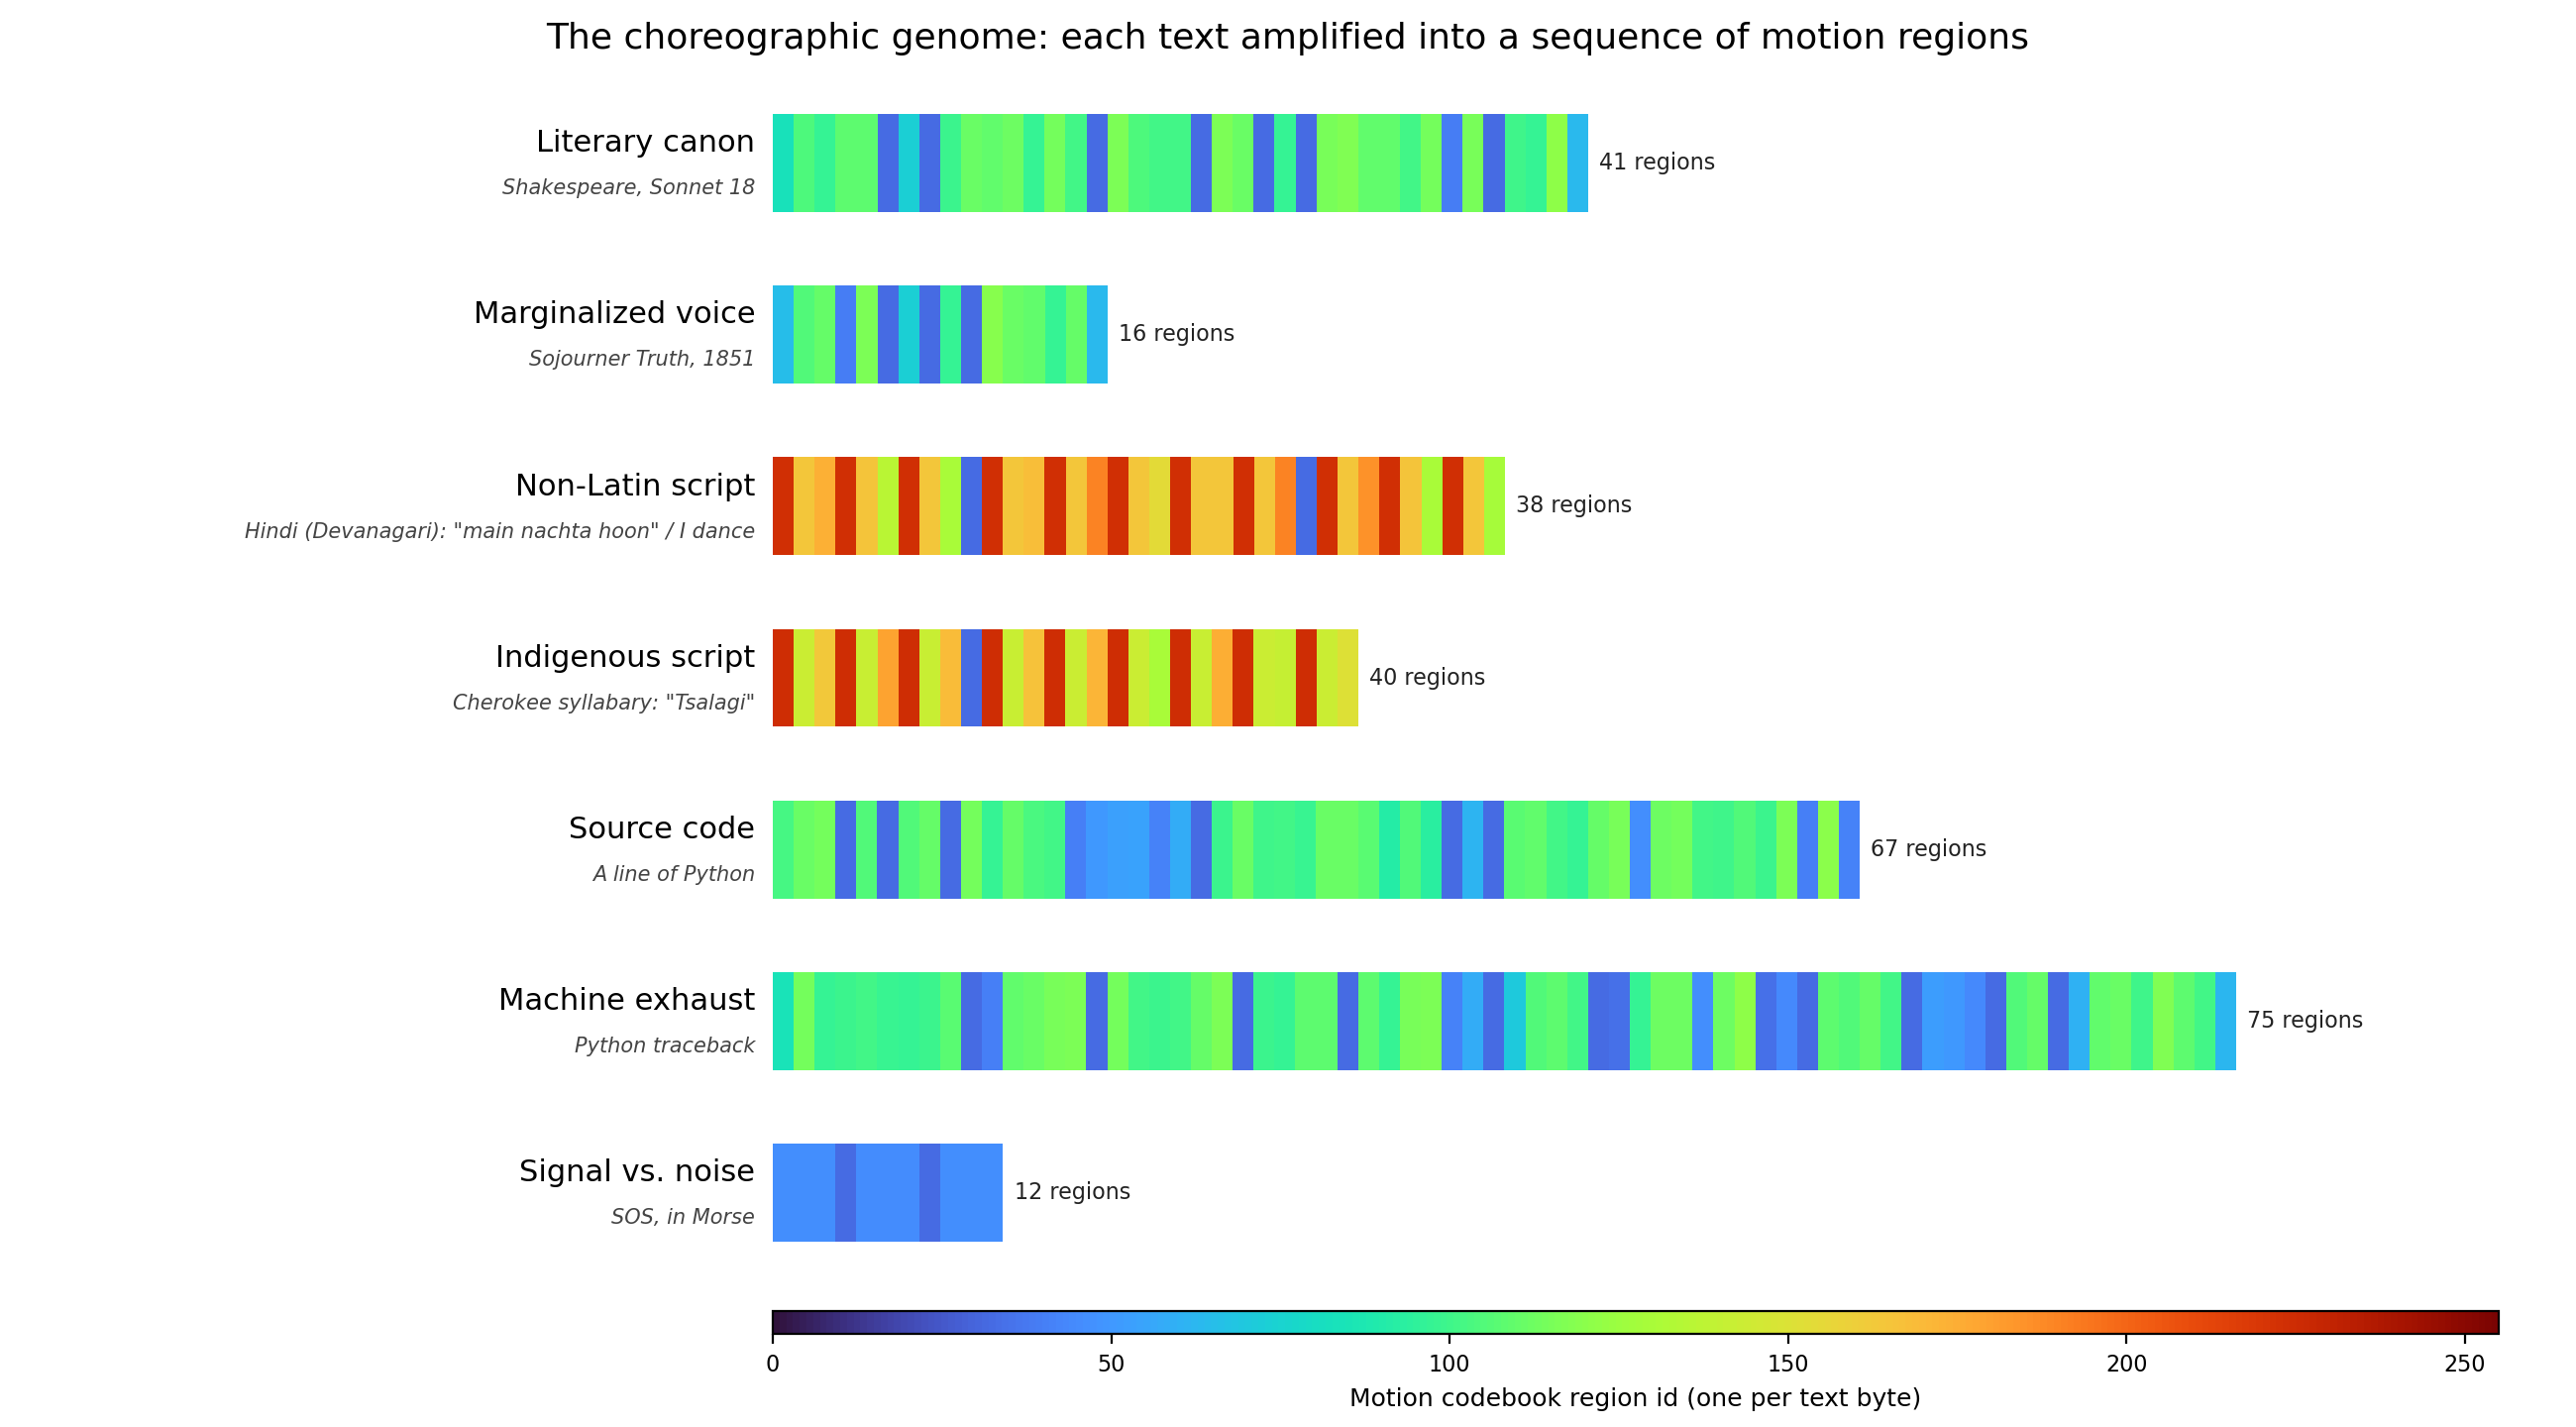
\includegraphics[width=0.95\linewidth]{plot_5_choreographic_genome}
  \caption{The ``choreographic genome''. Each text is amplified, byte by byte, into
  a sequence of motion regions, where color encodes region ID (\cref{eq:amp}).
  Because UTF-8 spends more bytes on non-Latin scripts, the Devanagari and Cherokee
  strips run long and warm despite their short character counts, while the ``SOS''
  distress call collapses into a brief, repetitive pulse. Each text yields a
  visibly distinct genome, with a mean pairwise edit distance of 44.3 across the
  corpus.}
  \label{fig:genome}
\end{figure*}

\section{Amplifying Texts: Artistic Case Studies}
\label{sec:cases}

To study the instrument as a visualization rather than as a benchmark, we
assembled a deliberately heterogeneous corpus spanning many themes: the loud Western canon, the overlooked exhaust of machines,
historically marginalized voices, and scripts that digital infrastructure was
never centered on. For each text, we compute its genome and measure the movement
required to physically realize it. \Cref{tab:cases} reports the results, and
\cref{fig:genome,fig:amp,fig:montage,fig:trail} visualize them.

\begin{table}[tb]
\caption{Structural amplification across the case-study corpus. ``Regions'' counts
the motion gestures the body traverses (bytes plus bridges inserted for physical
continuity); ``amplification'' is regions per source character; ``entropy'' is over
the region distribution.}
\label{tab:cases}
\centering
\footnotesize
\setlength{\tabcolsep}{4.5pt}
\begin{tabular}{@{}lrrrr@{}}
\toprule
Text (register)            & Chars & Regions & Amp./char & Entropy \\
\midrule
Sonnet (canon)             & 39 & 41 & 1.05 & 3.94 \\
Sojourner Truth (margin.)  & 16 & 16 & 1.00 & 3.45 \\
Hindi / Devanagari         & 13 & 38 & 2.92 & 2.86 \\
Cherokee (Indigenous)      & 10 & 40 & 4.00 & 3.09 \\
Source code (Python)       & 52 & 67 & 1.29 & 4.53 \\
Traceback (machine)        & 70 & 75 & 1.07 & 4.49 \\
SOS / Morse                & 11 & 12 & 1.09 & 1.44 \\
\bottomrule
\end{tabular}
\end{table}

\subsection{Every text has a body}
The genomes in \cref{fig:genome} are immediately and legibly different from one
another. This confirms the instrument's basic claim: structure alone, with meaning
withheld, is enough to give every text a distinct physical identity. Across the
corpus, the mean pairwise edit distance between genomes is 44.3 regions, which
quantitatively supports what the figure shows. Furthermore, because the
byte-to-region mapping is fully deterministic, the same text always yields the same
genome, so this structural identity is stable and repeatable. The engine then
realizes that genome through motion matching, selecting specific frames and, where
needed, bridging regions to keep the body continuous; the exact frames of any
single performance depend on that search and can vary between runs. It is therefore
the genome, rather than any single performance, that serves as the text's
fingerprint. \Cref{fig:teaser} makes the point at a glance, presenting one
characteristic pose for each of the seven texts.

\subsection{Amplifying what ASCII marginalizes}
The most pointed result is also the simplest. ASCII English spends roughly one
byte per character, so the canonical and the marginalized English texts amplify at
approximately one region per character. However, UTF-8 spends two to four bytes on
the scripts it treats as exceptions to a Latin default. The Devanagari phrase
meaning ``I dance'' (13 characters) and a Cherokee phrase (10 characters)
therefore unfold into 38 and 40 regions, which are amplification factors of 2.9
and 4.0 (\cref{fig:amp}). \Cref{fig:trail} visualizes this directly, presenting the
full generated dance for the Devanagari phrase as a single chronophotographic
sweep; the instrument never reads that the phrase means ``I dance'', yet the byte
structure alone produces a complete choreographic arc. The very encoding overhead
that makes these scripts ``expensive'' and peripheral to computing becomes, in our
instrument, a surplus of embodied expression: the overlooked script is given more
body, not less. We are careful not to overstate this result. The system does not
understand these languages, and its movement vocabulary carries its own cultural
biases, which we discuss in \cref{sec:discussion}. However, the inversion is real
and demonstrable, and we find it a productive provocation, a visualization in which
the cost of marginalization is re-read as amplitude.

\begin{figure*}[!t]
  \centering
  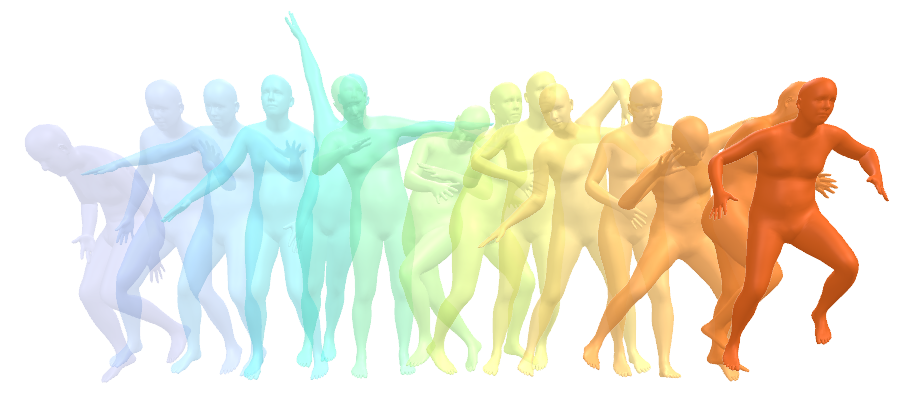
\includegraphics[width=0.92\linewidth]{plot_9_trail}
  \caption{A chronophotographic view of a single generated dance. We sample one
  sequence across time, spread the frames from left to right, and color them from
  cool to warm by moment. The entire sweep is produced from the byte structure of
  the Devanagari phrase meaning ``I dance''; the instrument never reads that
  meaning, yet the structure alone yields a complete choreographic arc.}
  \label{fig:trail}
\end{figure*}

\subsection{The dance of a sonnet versus an error log}
\Cref{fig:montage} renders three texts as time-sampled keyframes from the same
engine, and the contrast is borne out in the body. The sonnet, built from
lowercase Latin letters that cluster in a narrow byte range, moves in relatively
legato and recurring postures. The Python traceback, which mixes punctuation,
digits, mixed case, and the bracketed debris of a crash, carries one of the
highest structural entropies in the corpus (4.49 bits) and reads as jagged and
percussive, a body stuttering through exception handling. The Cherokee syllabary,
composed entirely of high continuation bytes, sweeps through the high regions of the
codebook in long and dense phrases. Thus, the same instrument, given
three different structures, choreographs three visibly different bodies.

\subsection{What counts as signal}
Our corpus also probes the the question of what a signal actually means. ``SOS'' in Morse is a
message that is nothing but a call to be heard, and it holds almost no lexical
content. Yet the instrument gives it the lowest-entropy genome in the set (1.44
bits): a short, insistent, repeating pulse (\cref{fig:genome}, bottom row). A
semantic model would find nothing to say about three dots, three dashes, and three
dots. Our structural amplifier instead produces a clear rhythmic signature. This
raises the question of which of the two systems has actually registered the signal.

\begin{figure*}[!t]
  \centering
  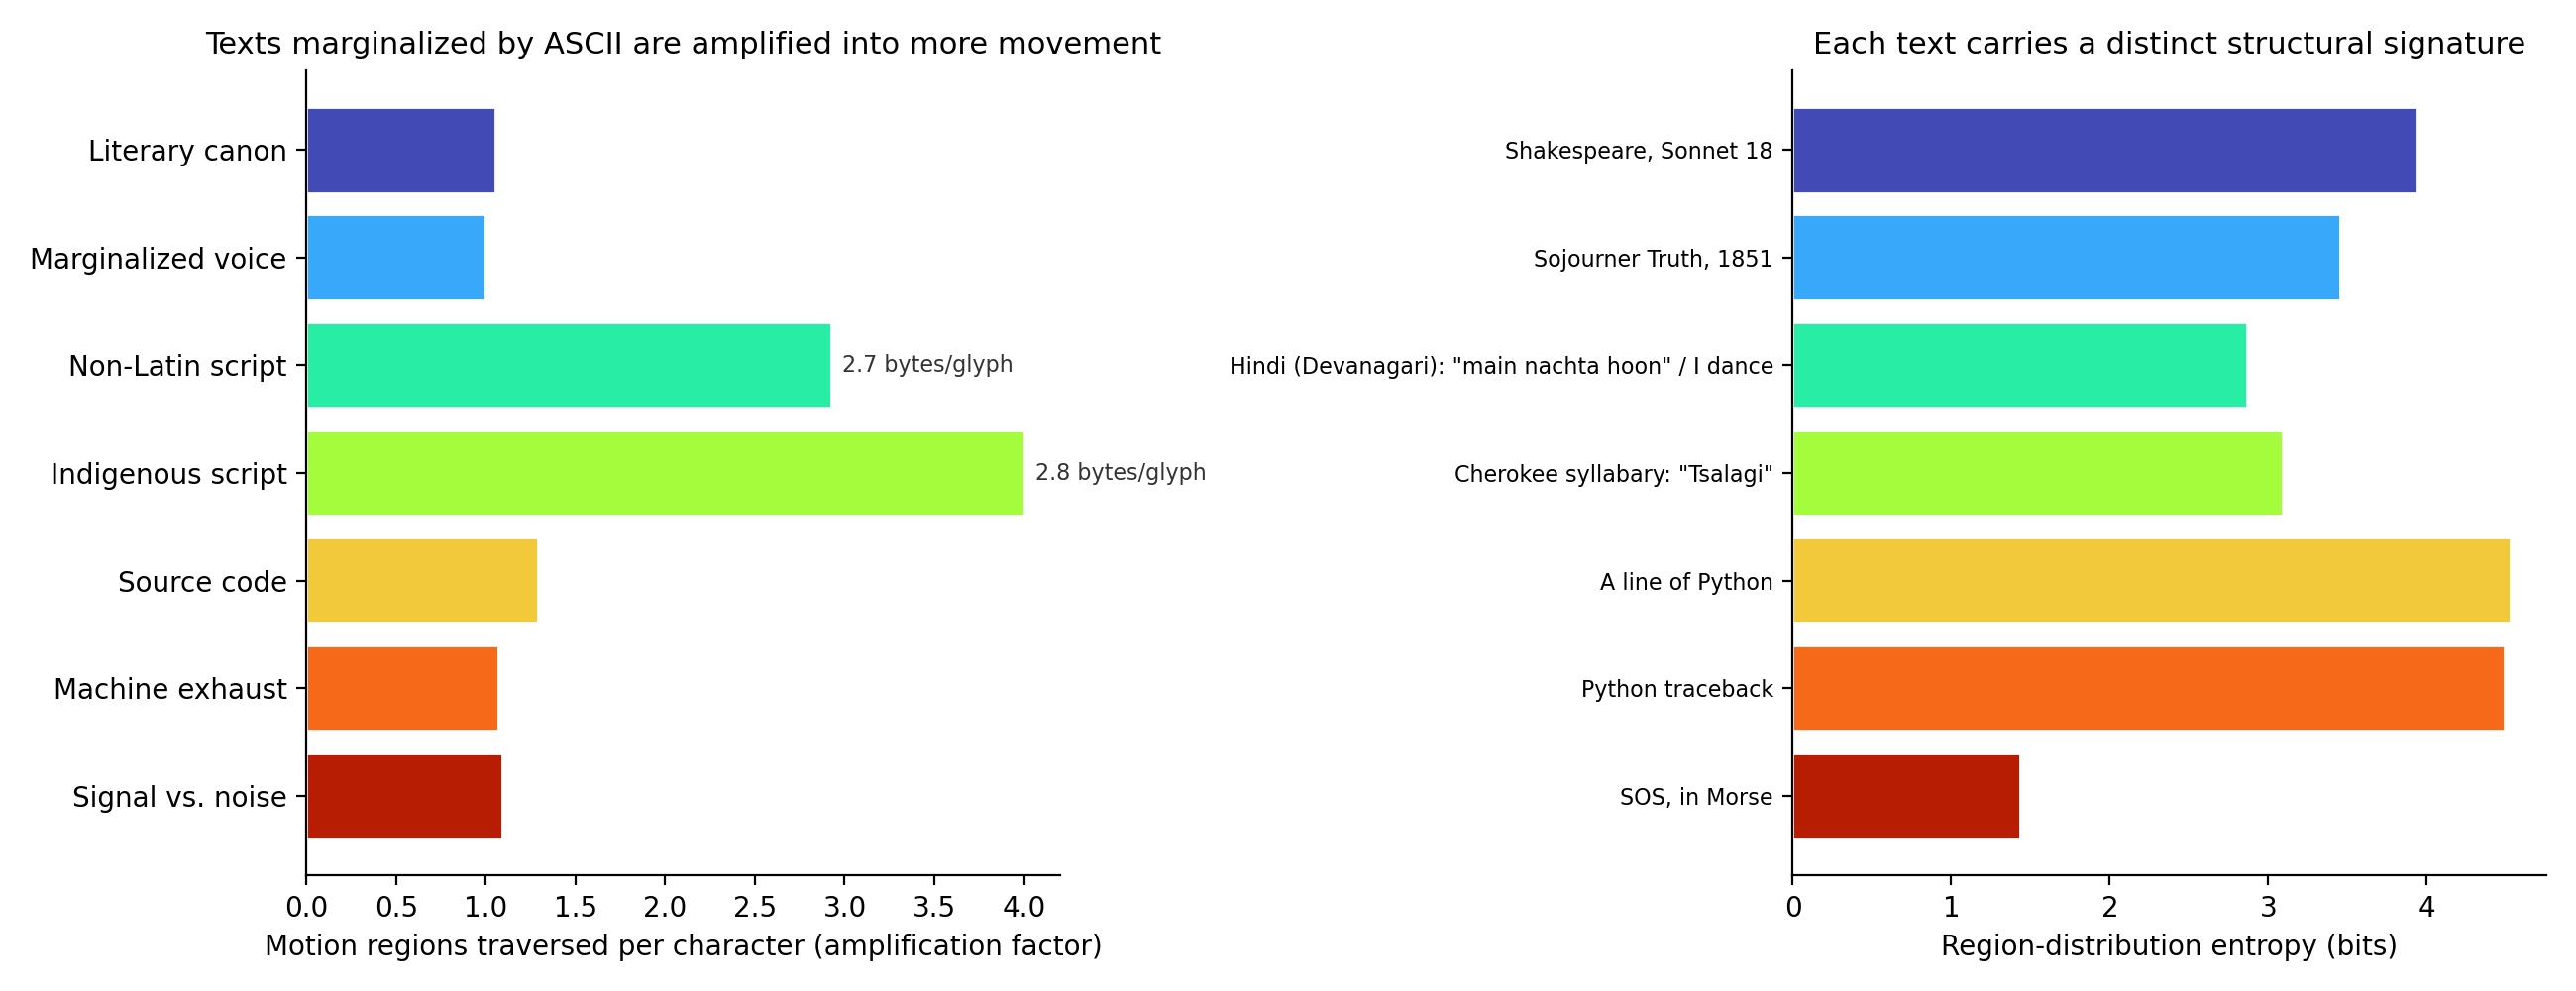
\includegraphics[width=0.95\linewidth]{plot_6_amplification}
  \caption{Left: motion regions traversed per character. Texts in scripts that
  UTF-8 encodes with several bytes per glyph are amplified into markedly more
  movement. Right: each text's region-distribution entropy, which is its structural
  signature. Source code and machine exhaust are the most varied, while the Morse
  distress call is the most repetitive.}
  \label{fig:amp}
\end{figure*}

\begin{figure*}[!t]
  \centering
  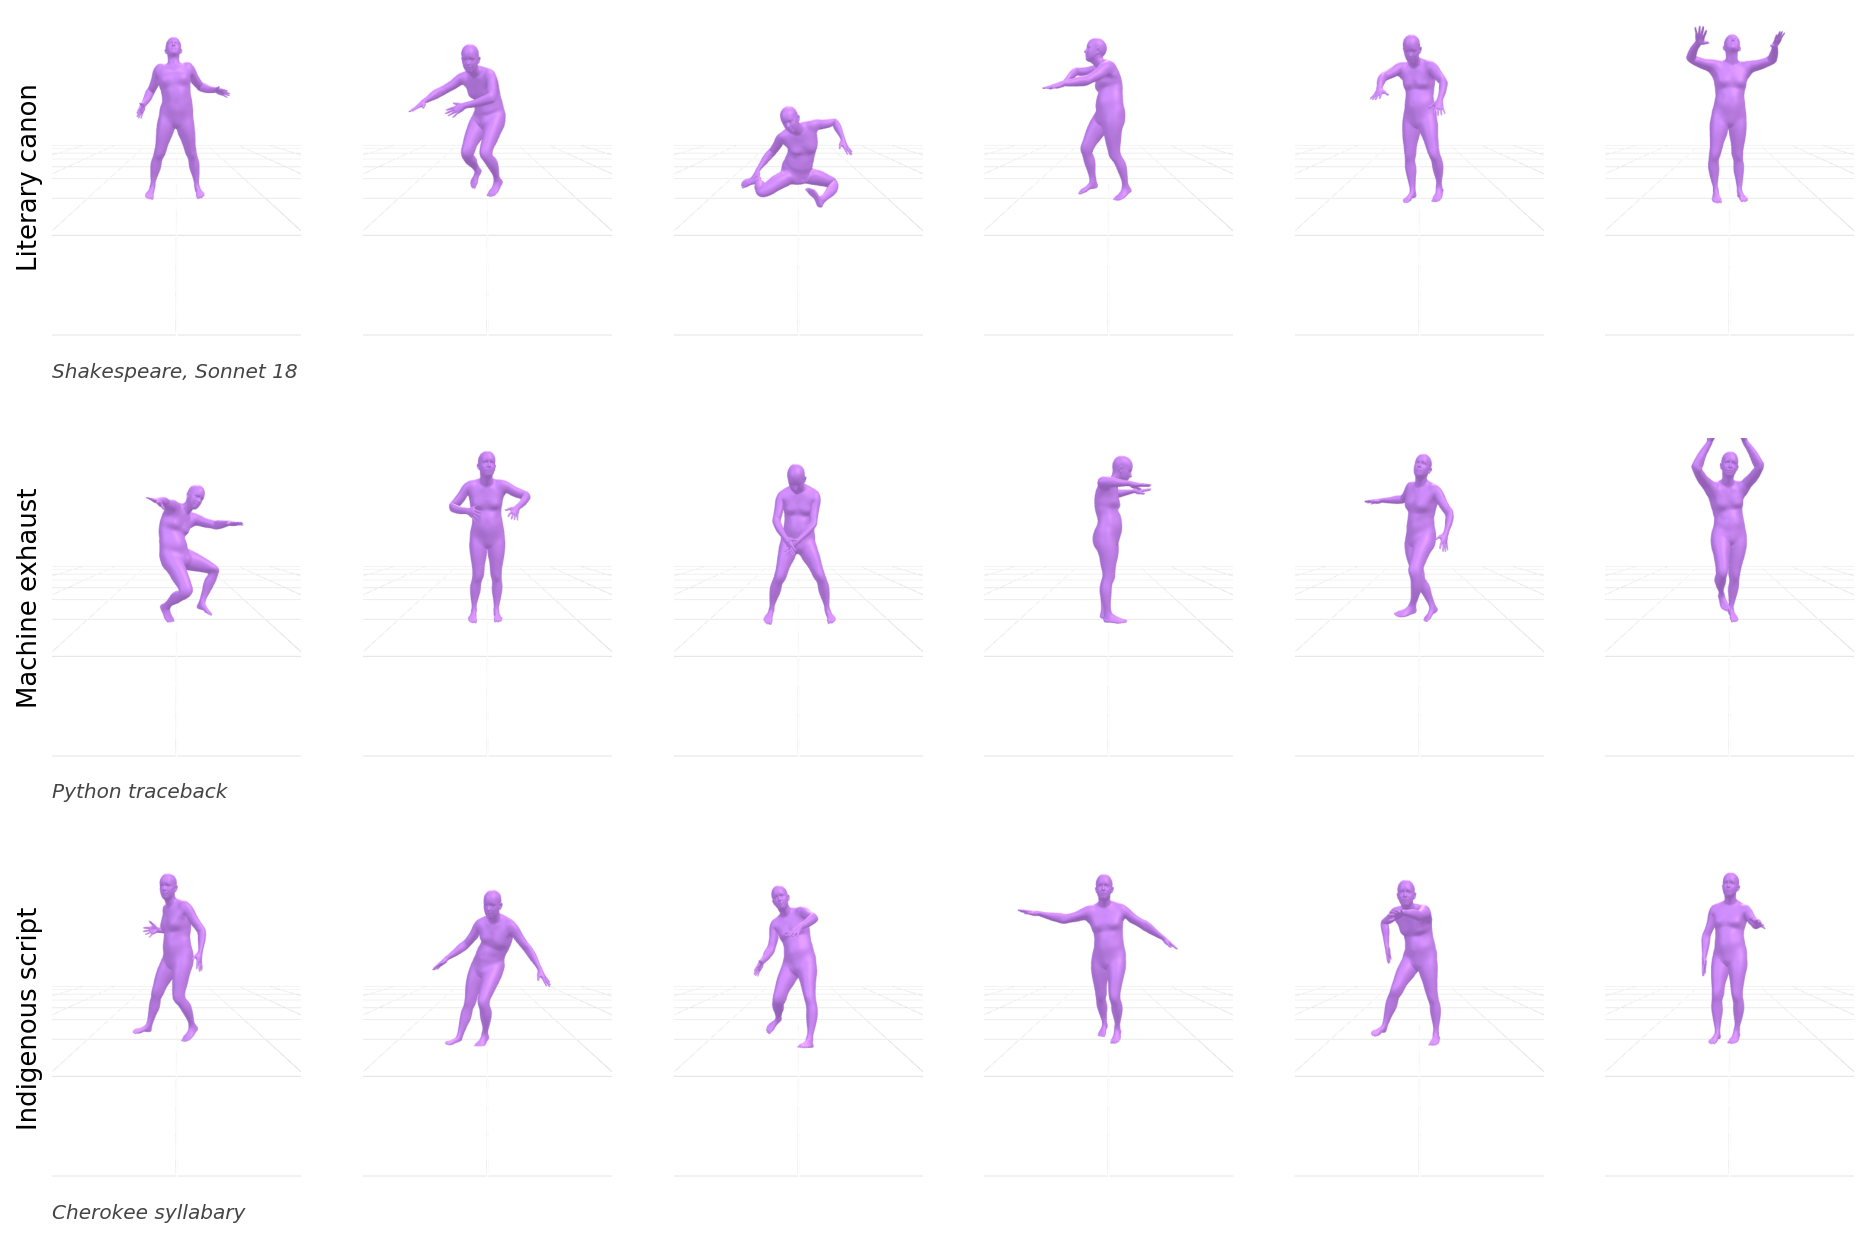
\includegraphics[width=0.95\linewidth]{plot_7_dance_montage}
  \caption{Physicalized choreography: time-sampled keyframes from the same
  engine driven by three different texts. The sonnet (top) is comparatively legato,
  the machine traceback (middle) is percussive and high in entropy, and the
  Cherokee syllabary (bottom) moves through long, dense phrases. These are renders
  of the actual generated motion, not schematic illustrations.}
  \label{fig:montage}
\end{figure*}

\section{Does the Instrument Work?}
\label{sec:validation}

Amplification is only meaningful if the instrument is faithful and the body it
drives is convincing. We therefore report a compact technical validation, and we
keep it deliberately brief. First, on invention: the sequences generated from text
contain choreographic phrases that are almost entirely absent from the training
corpus, with $99.9\%$ of three-gram and $100\%$ of four-gram region transitions
novel relative to AIST++. This confirms that the instrument composes rather than
retrieves. Second, on distinctness: genomes generated from different inputs diverge
sharply, with a mean region-sequence edit distance of $32.5$ over a random sample,
and text-driven motion carries a markedly higher mean kinetic energy than the
training data ($0.43$ versus $0.07$). This demonstrates that amplifying a text's
structure forces the body through dynamic changes of tempo. Third, on
traversability: the plausibility graph connects $54\%$ of all region pairs
directly, and Dijkstra bridging keeps detours short, with a mean of $0.59$ inserted
bridges per transition and most transitions requiring none. Finally, on fluidity:
the physics layer reduces foot-skating from $0.121$ to $0.010$ and jerk from
$1.2\times10^{-2}$ to $8.9\times10^{-4}$, the latter below the AIST++ baseline
itself, with negligible floor penetration. The instrument is therefore both
inventive and physically credible.

\section{Discussion}
\label{sec:discussion}

The central contribution of this work is less the pipeline than the inversion it
embodies. Semantic generation amplifies the part of language that is already loud,
its sanctioned meaning, and in doing so it reproduces the biases of whoever
assembled the training data~\cite{crawford2021atlas,dignazio2020datafeminism}. By
amplifying structure instead, our instrument turns up a signal that is present in
every text but attended to in almost none, and it does so on equal terms for a
sonnet and a stack trace. In this sense, the moving body becomes an instrument that
makes the quiet material of data legible.

At the same time, amplification is never neutral, and we resist a triumphant
reading of our own results. The movement vocabulary is learned from AIST++, a
corpus of largely studio street dance, so the body that speaks every text is
culturally specific, and the equal treatment we claim holds only with respect to
that vocabulary. Furthermore, the amplification of multibyte scripts is a property
of UTF-8, not evidence of any understanding of the languages it encodes; the
instrument can give Cherokee more movement without knowing a single word of
Cherokee. We consider this honesty to be part of the work, because an amplifier
that concealed its own coloration would be exactly the kind of system this project
sets out to question.

Because the core of the instrument is classical and interpretable, an artist can
actually read it. The genome is legible, the bridges are logged, and the same text
reliably yields the same genome, which the engine can replay exactly when its
random seed is fixed. This makes the system a partner that an artist can
play and argue with, rather than an oracle that must be trusted, which is closer to
an instrument than to an autocomplete. We imagine performers ``playing'' texts in
real time, curators amplifying archival documents into embodied form, and
communities choreographing words in scripts that mainstream models still render as
empty boxes.

Finally, the natural home of this work is spatial and temporal. Beyond the page,
the instrument supports a gallery installation in which audience-supplied texts are
amplified into projected choreography in real time, as well as a multi-screen piece
that sets the dances of canonical and overlooked texts side by side. Supplementary
video renders accompany this submission. In future work, we plan to expand the
behavioral codebook with more diverse kinetic datasets, such as classical ballet or
everyday movement, in order to broaden the vocabulary of the body and to loosen the
cultural specificity discussed above.

\section{Conclusion}
In this work, we presented an embodied visualization instrument that amplifies the
hidden structure of text into movement. By mapping raw bytes onto a quantized
vocabulary of gesture and refusing to interpret meaning, the system turns the
dancing body into a display for the quiet, material signal that semantics-first
generation discards. Across a corpus of canonical, marginalized, machine, and
Indigenous texts, it renders each input as a distinct choreographic genome, and it
amplifies the scripts that our infrastructure overlooks into more, rather than
less, embodied expression. Ultimately, we offer this instrument less as a better
way to make dances than as a way to ask, of any data stream, what we have chosen
to hear, and what we might choose to amplify instead.

\section{AI Incorporation and Usage}
The artwork is a generative system by design; the choreography in every figure is produced algorithmically by the pipeline described in \cref{sec:system}. The authors curated the inputs and the framing rather than
individual keyframes. The code was mostly written by a combination of GitHub Copilot and Claude Code, but prompts and ideas came from humans. We deliberately use classical, interpretable machine
learning, specifically PCA, K-Means, and graph search, rather than a large neural
generator, for sake of interpretability.

AI assistance was utilized for initial drafting purposes, most notably for literature review and result analysis. A combination of Gemini and Claude Code were used. All AI drafted content has been reviewed and edited by the authors, and the authors take full responsibility for the writing.

\section*{Supplemental Materials}
\label{sec:supplemental_materials}
The source code, the motion codebook and plausibility graph, the case-study
corpus, and supplementary video renders of the choreography are available at
\url{https://github.com/ML72/Choreographic-Genome}, with a visual demo at
\url{https://ml72.github.io/Choreographic-Genome/}. All figures in this paper were
generated by the system described here, and no figure is reproduced from another
source.

\acknowledgments{
We gratefully acknowledge the instructors of the Art and Machine Learning (10-615) course at Carnegie Mellon University in Spring 2026, whose insightful lectures sparked the initial inspiration for this project. We also thank the creators of the AIST++ dataset for making this work possible.}

\bibliographystyle{abbrv-doi}
\bibliography{references}

\end{document}
